\documentclass[11pt,a4paper]{article}
\usepackage[utf8]{inputenc}
\usepackage[T1]{fontenc}
\usepackage{amsfonts}
\usepackage{amssymb}
\usepackage{mdframed}
\usepackage{tikz}
\usetikzlibrary{calc}
\usepackage{tkz-tab}
\usepackage{pgfplots}
\usepackage{xcolor}
\usepackage{fancyhdr}
\usepackage{lastpage}
\usepackage[fleqn]{amsmath}
\setlength{\mathindent}{0pt}

\newcommand{\pdt}{\mathbin{\vcenter{\hbox{\scalebox{0.6}{\textbullet}}}}}


% Spécifications du document
\newcommand{\doctitre}{Produit scalaire et applications} % Ex: Le second degré
\newcommand{\docniveau}{$1^{\text{re}}$ Spécialité mathématiques} % Ex: 1^{\text{re}}$ Spécialité mathématiques
\newcommand{\doctheme}{Géométrie} %Ex: Algèbre
\newcommand{\doctype}{Démonstrations} % Ex: Démonstrations
\newcommand{\docshorttype}{Démo} % Démo

% Couleurs pour les graphiques
\definecolor{dark_green}{HTML}{008000}

% Paramètres du document
\RequirePackage{geometry}
\geometry{tmargin=1cm,bmargin=1.9cm,lmargin=1.9cm,rmargin=1.9cm}
\renewcommand{\familydefault}{\sfdefault}
\setlength{\parindent}{0pt}
\title{\doctitre}
\author{\docniveau \\ \doctheme\text{ - }\doctype}
\date{}
\fancypagestyle{custom}{
  \fancyhf{}
  \renewcommand{\headrulewidth}{0pt}
  \lfoot{\doctheme\text{ - }\docshorttype}
  \cfoot{\doctitre} % Change \titre to \doctitre
  \rfoot{\thepage/\pageref{LastPage}}
}

% Styles pour les mdframed
\mdfdefinestyle{definitionStyle}{
    leftline=true,
    rightline=false,
    topline=false,
    bottomline=false,
    linewidth=2pt,
    linecolor=black,
    innertopmargin=0pt,
    innerbottommargin=0pt,
    innerrightmargin=0pt,
    innerleftmargin=5pt,
}

\mdfdefinestyle{proprieteStyle}{
    linewidth=1pt,
    linecolor=black,
    innertopmargin=5pt,
    innerbottommargin=5pt,
    innerrightmargin=5pt,
    innerleftmargin=5pt,
}
% ----- DEBUT DU DOCUMENT -----
\begin{document}

% Style et numérotation
\maketitle
\pagestyle{custom}
\thispagestyle{custom}

\section*{I. Premières expressions du produit scalaire de deux vecteurs}

\subsection*{2. Formule du projeté orthogonal}

\underline{Démonstration \emph{(expression du produit sclaire n°2)} :}

\begin{itemize}
    \item Premier cas : \\
          \begin{tikzpicture}[scale=1,>=stealth]
              \draw[] (-1,0) (5,0) ;
              \coordinate (A1) at (0,0);
              \coordinate (B1) at (3,0);
              \coordinate (C1) at (2,2);
              \coordinate (H1) at (2,0);
              \draw[->,thick,red] (A1) -- (C1) node[midway,anchor=south east] {$\vec{v}$};
              \draw[->,thick,blue] (A1) -- (B1) node[midway,anchor=north east] {$\vec{u}$};
              \draw[thick,dark_green, dashed] (C1) -- (H1) node[midway,anchor=north east] {};
              \draw[line width=0.6pt] (A1) ++(-0.05,-0.05) -- ++(0.1,0.1) (A1) ++(-0.05,0.05) -- ++(0.1,-0.1) node[anchor=south east] {$A$};
              \draw[line width=0.6pt] (B1) ++(-0.05,-0.05) -- ++(0.1,0.1) (B1) ++(-0.05,0.05) -- ++(0.1,-0.1) node[anchor=south] {$B$};
              \draw[line width=0.6pt] (C1) ++(-0.05,-0.05) -- ++(0.1,0.1) (C1) ++(-0.05,0.05) -- ++(0.1,-0.1) node[anchor=south west] {$C$};
              \draw[line width=0.6pt] (H1) ++(-0.05,-0.05) -- ++(0.1,0.1) (H1) ++(-0.05,0.05) -- ++(0.1,-0.1) node[anchor=south east] {$\color{dark_green}H$};
              \draw[thick,dark_green] (2.2,0) -- (2.2,0.2) node[midway,anchor=north east] {};
              \draw[thick,dark_green] (2,0.2) -- (2.2,0.2) node[midway,anchor=north east] {};
          \end{tikzpicture}
          \text{ } \\
          $\overrightarrow{AB}\pdt\overrightarrow{AC}=AB\times AC\times\cos{(\widehat{BAC})}$ \\
          Dans le triangle $ACH$ rectangle en $H$, $\cos{(\widehat{BAC})}=\frac{AH}{AC}$
          \vspace{-6pt}
          \begin{equation*}
              \begin{split}
                  \text{Donc }\overrightarrow{AB}\pdt\overrightarrow{AC} & =AB\times AC \times \frac{AH}{AC} \\
                  &=AB\times AH
              \end{split}
          \end{equation*}
          Or $\overrightarrow{AB}\pdt\overrightarrow{AH}=AB\times AH$ \\
          Donc $\overrightarrow{AB}\pdt\overrightarrow{AC}=\overrightarrow{AB}\pdt\overrightarrow{AH}$
    \item Deuxième cas : \\
          \begin{tikzpicture}[scale=1,>=stealth]
              \draw[] (-1,0) (5,0) ;
              \coordinate (A2) at (2,0);
              \coordinate (B2) at (5,0);
              \coordinate (C2) at (0.5,1.5);
              \coordinate (H2) at (0.5,0);
              \draw[->,thick,blue] (A2) -- (B2) node[midway,anchor=north] {$\vec{u}$};
              \draw[->,thick,red] (A2) -- (C2) node[midway,anchor=south west] {$\vec{v}$};
              \draw[thick,dark_green, dashed] (C2) -- (H2) node[midway,anchor=north east] {};
              \draw[thick,blue, dashed] (A2) -- (H2) node[midway,anchor=north east] {};
              \draw[line width=0.6pt] (A2) ++(-0.05,-0.05) -- ++(0.1,0.1) (A2) ++(-0.05,0.05) -- ++(0.1,-0.1) node[anchor=north east] {$A$};
              \draw[line width=0.6pt] (B2) ++(-0.05,-0.05) -- ++(0.1,0.1) (B2) ++(-0.05,0.05) -- ++(0.1,-0.1) node[anchor=north] {$B$};
              \draw[line width=0.6pt] (C2) ++(-0.05,-0.05) -- ++(0.1,0.1) (C2) ++(-0.05,0.05) -- ++(0.1,-0.1) node[anchor=south east] {$C$};
              \draw[line width=0.6pt] (H2) ++(-0.05,-0.05) -- ++(0.1,0.1) (H2) ++(-0.05,0.05) -- ++(0.1,-0.1) node[anchor=south east] {$\color{dark_green}H$};
              \draw[thick,dark_green] (0.7, 0) -- (0.7,0.2) node[midway,anchor=north east] {};
              \draw[thick,dark_green] (0.5, 0.2) -- (0.7,0.2) node[midway,anchor=north east] {};
          \end{tikzpicture}
          \text{ } \\
          $\overrightarrow{AB}\pdt\overrightarrow{AC}=AB\times AC\times\cos{(\widehat{BAC})}$ \\
          Dans le triangle $ACH$ rectangle en $H$, $\cos{(\widehat{BAC})}=\frac{AH}{AC}$. \\
          Or, $\widehat{CAH}=180^\circ -\widehat{BAC}$ et $\cos{(\widehat{CAH})}=\cos{(180^\circ-\widehat{BAC})}=-\cos{(\widehat{BAC})}$ \\
          \vspace{-6pt}
          \begin{equation*}
              \begin{split}
                  \text{Ainsi, }\overrightarrow{AB}\pdt\overrightarrow{AC} & =AB\times AC \times (-\cos{(\widehat{CAH})}) \\
                  &=-AB\times AC\times\frac{AH}{AC} \\
                  &=-AB\times AH
              \end{split}
          \end{equation*}
          \vspace{-6pt}
          \begin{equation*}
              \begin{split}
                  \text{Or, }\overrightarrow{AB}\pdt\overrightarrow{AH} & =AB\times AH \times \cos{(180^\circ)} \\
                  &=-AB\times AH
              \end{split}
          \end{equation*}
          Donc $\overrightarrow{AB}\pdt\overrightarrow{AC}=\overrightarrow{AB}\pdt\overrightarrow{AH}$
\end{itemize}

\newpage

\section*{II. Propriétés du produit scalaire}

\subsection*{1. Symétrie et bilinéarité}

\underline{Démonstration \emph{(symétrie)} :}

\begin{equation*}
    \begin{split}
        \vec{u}\pdt\vec{v}&=\|\vec{u}\|\times\|\vec{v}\|\times\cos{(\vec{u}, \vec{v})} \\
        \vec{v}\pdt\vec{u}&=\|\vec{v}\|\times\|\vec{u}\|\times\cos{(\vec{v}, \vec{u})}
    \end{split}
\end{equation*}
$\cos{(\vec{u}, \vec{v})}=\cos{(\vec{v}, \vec{u})}$ \\
Donc $\vec{u}\pdt\vec{v}=\vec{v}\pdt\vec{u}$
\subsection*{2. Expression du produit scalaire dans un repère orthonormé}

\underline{Démonstration \emph{(expression du produit scalaire n°3)} :}~\\

Soit $\displaystyle\vec{u}\binom{x}{y}$ et $\displaystyle\vec{v}\binom{x'}{y'}$ deux vecteurs dans un repère orthonormé $(O, I, J)$.

\begin{minipage}{0.25\textwidth}
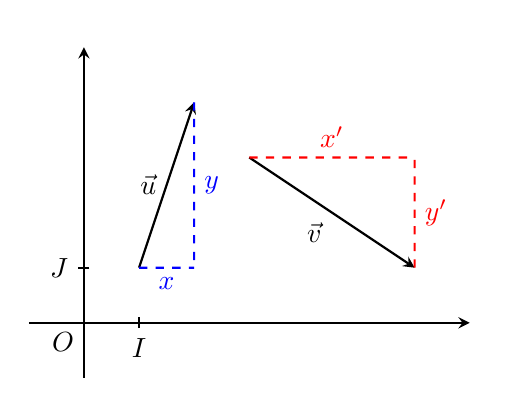
\begin{tikzpicture}[scale=0.7,>=stealth]
    % Axes
    \draw[->, thick] (-1, 0) -- (7, 0) node[anchor=west] {};
    \draw[->, thick] (0, -1) -- (0, 5) node[anchor=south] {};

    % Points
    \coordinate (A) at (1,1);
    \coordinate (B) at (2,4);
    \coordinate (C) at (3,3);
    \coordinate (D) at (6,1);
    
    % Vecteurs u et v
    \draw[->, thick, black] (A) -- (B) node[midway, anchor=east] {$\vec{u}$};
    \draw[thick, blue, dashed] (A) -- (2, 1) node[midway,anchor=north] {$x$};
    \draw[thick, blue, dashed] (B) -- (2, 1) node[midway,anchor=west] {$y$};
    
    
    \draw[->, thick, black] (C) -- (D) node[midway, anchor=north east] {$\vec{v}$};
    \draw[thick, red, dashed] (C) -- (6, 3) node[midway,anchor=south] {$x'$};
    \draw[thick, red, dashed] (D) -- (6, 3) node[midway,anchor=west] {$y'$};
    
    % Marquer le repère
    \node[anchor=north east] at (0, 0) {$O$};
    \draw[thick] (1, 0.1) -- (1, -0.1) node[anchor=north] {$I$};
    \draw[thick] (0.1, 1) -- (-0.1, 1) node[anchor=east] {$J$};
\end{tikzpicture}
\end{minipage}
\hfill
\begin{minipage}{0.64\textwidth}
    \begin{equation*}
        \begin{split}
            \text{On a } & \vec{u}=x\overrightarrow{OI} + y\overrightarrow{OJ} \\
        & \vec{v}=x'\overrightarrow{OI} + y'\overrightarrow{OJ}
    \end{split}
\end{equation*}
\begin{equation*}
    \begin{split}
        \text{Calculons } \vec{u}\pdt\vec{v} &= (x\overrightarrow{OI} + y\overrightarrow{OJ}) \pdt (x'\overrightarrow{OI} + y'\overrightarrow{OJ}) \\
        &= x\overrightarrow{OI}\pdt x'\overrightarrow{OI} + x\overrightarrow{OI}\pdt y'\overrightarrow{OJ} + y\overrightarrow{OJ}\pdt x'\overrightarrow{OI} + y\overrightarrow{OJ}\pdt y'\overrightarrow{OJ} \\
        &= xx'\overrightarrow{OI}\pdt \overrightarrow{OI} + xy'\overrightarrow{OI}\pdt\overrightarrow{OJ} + yx'\overrightarrow{OJ}\pdt\overrightarrow{OI} + yy'\overrightarrow{OJ}\pdt\overrightarrow{OJ} \\
        &= xx'\times1+0+0+yy'\times1 \\
        & = xx'+yy'
    \end{split}
\end{equation*}
\end{minipage}

\subsection*{3. Identités remarquables avec le produit scalaire}

\underline{Démonstrations \emph{(identités remarquables concernant le produit scalaire)} :}

\begin{itemize}
    \item Idendité remarquable n°1 :
    \begin{equation*}
        \begin{split}
            (\vec{u}+\vec{v})^2&=(\vec{u}+\vec{v})\pdt(\vec{u}+\vec{v}) \\
            &=\vec{u}\pdt\vec{u}+\vec{u}\pdt\vec{v}+\vec{v}\pdt\vec{u}+\vec{v}\pdt\vec{v} \\
            &=\|\vec{u}\|^2+\vec{u}\pdt\vec{v}+\vec{v}\pdt\vec{u}+\|\vec{v}\|^2\\
            &=\|\vec{u}\|^2+2\vec{u}\pdt\vec{v}+\|\vec{v}\|^2
        \end{split}
    \end{equation*}
    \item Idendité remarquable n°2 :
    \begin{equation*}
        \begin{split}
            (\vec{u}-\vec{v})^2&=(\vec{u}-\vec{v})\pdt(\vec{u}-\vec{v}) \\
            &=\vec{u}\pdt\vec{u}+\vec{u}\pdt(-\vec{v})-\vec{v}\pdt\vec{u}-\vec{v}\pdt(-\vec{v}) \\
            &=\|\vec{u}\|^2+\vec{u}\pdt(-\vec{v})-\vec{v}\pdt\vec{u}+\|\vec{v}\|^2\\
            &=\|\vec{u}\|^2-2\vec{u}\pdt\vec{v}+\|\vec{v}\|^2
        \end{split}
    \end{equation*}
    \item Idendité remarquable n°3 :
    \begin{equation*}
        \begin{split}
            (\vec{u}+\vec{v})\pdt(\vec{u}-\vec{v})&=\vec{u}\pdt\vec{u}+\vec{u}\pdt(-\vec{v})+\vec{v}\pdt\vec{u}+\vec{v}\pdt(-\vec{v}) \\
            &=\|\vec{u}\|^2+\underbrace{\vec{u}\pdt(-\vec{v})+\vec{v}\pdt\vec{u}}_{= \text{ }0}-\|\vec{v}\|^2 \\
            &=\|\vec{u}\|^2-\|\vec{v}\|^2
        \end{split}
    \end{equation*}
\end{itemize}

\newpage

\underline{Démonstrations \emph{(conséquence des nouvelles expressions du produit scalaire)} :}

\begin{itemize}
    \item D'après l'identité remarquable n°1 :
    \begin{align*}
            &(\vec{u}+\vec{v})^2=\|\vec{u}\|^2+2\vec{u}\pdt\vec{v}+\|\vec{v}\|^2 \\
            \Leftrightarrow\text{ }&\|\vec{u}+\vec{v}\|^2=\|\vec{u}\|^2+2\vec{u}\pdt\vec{v}+\|\vec{v}\|^2 \\
            \Leftrightarrow\text{ }&\|\vec{u}+\vec{v}\|^2-\|\vec{u}\|^2-\|\vec{v}\|^2=-2\vec{u}\pdt\vec{v} \\
            \Leftrightarrow\text{ }&\frac{1}{2}\left( \|\vec{u}+\vec{v}\|^2-\|\vec{u}\|^2-\|\vec{v}\|^2\right)=\vec{u}\pdt\vec{v}
    \end{align*}
    \item D'après l'identité remarquable n°2 :
    \begin{align*}
            &(\vec{u}-\vec{v})^2=\|\vec{u}\|^2-2\vec{u}\pdt\vec{v}+\|\vec{v}\|^2 \\
            \Leftrightarrow\text{ }&\|\vec{u}-\vec{v}\|^2=\|\vec{u}\|^2-2\vec{u}\pdt\vec{v}+\|\vec{v}\|^2 \\
            \Leftrightarrow\text{ }&\|\vec{u}-\vec{v}\|^2-\|\vec{u}\|^2-\|\vec{v}\|^2=-2\vec{u}\pdt\vec{v} \\
            \Leftrightarrow\text{ }&-\|\vec{u}-\vec{v}\|^2+\|\vec{u}\|^2+\|\vec{v}\|^2=2\vec{u}\pdt\vec{v} \\
            \Leftrightarrow\text{ }&\frac{1}{2}\left(\|\vec{u}\|^2+\|\vec{v}\|^2 - \|\vec{u}-\vec{v}\|^2\right)=\vec{u}\pdt\vec{v}
    \end{align*}
    \item D'après les identités remarquables n°1 et n°2 :
    \begin{align*}
        &\frac{1}{4}\left( \|\vec{u}+\vec{v}\|^2 - \|\vec{u}-\vec{v}\|^2 \right) \\
        =& \frac{1}{4} \left( \|\vec{u}\|^2+\|\vec{v}\|^2+2\vec{u}\pdt\vec{v} -  (\|\vec{u}\|^2+\|\vec{v}\|^2-2\vec{u}\pdt\vec{v}) \right) \\
        =& \frac{1}{4} \left( \|\vec{u}\|^2+\|\vec{v}\|^2+2\vec{u}\pdt\vec{v} - \|\vec{u}\|^2-\|\vec{v}\|^2+2\vec{u}\pdt\vec{v} \right) \\
        =&\frac{1}{4}\left( 4\vec{u}\pdt\vec{v} \right) = \vec{u}\pdt\vec{v}
\end{align*}
\end{itemize}


\subsection*{4. Orthogonalité}

\underline{Démonstration :} ~\\

Soit $\vec{u}$ et $\vec{v}$ deux vecteurs non nuls et $A$, $B$ et $C$ trois points distincts tels que $\vec{u}=\overrightarrow{AB}$ et $\vec{v}=\overrightarrow{AC}$. \\

Si $\vec{u}$ et $\vec{v}$ sont orthogonaux alors $\widehat{BAC}=90^\circ$ donc $\cos{(\widehat{BAC})}=0$ donc $\vec{u}\pdt\vec{v}=\|\vec{u}\|\times\|\vec{v}\|\times\cos{(\widehat{BAC})}=0$. \\

Si $\vec{u}\pdt\vec{v}=0$ alors $\|\vec{u}\|\times\|\vec{v}\|\times\cos{(\widehat{BAC})}=0$. \\
Or $\|\vec{u}\|\not=0$ et $\|\vec{v}\|\not=0$. \\
Donc $\cos{(\widehat{BAC})}=0$. \\
Donc $\widehat{BAC}=90^\circ$. \\

Donc  $\vec{u}$ et $\vec{v}$ sont orthogonaux. \\


\underline{Démonstration \emph{(critère d'orthogonalité dans un repère orthonormé)} :}
\begin{align*}
    &\vec{u} \text{ et } \vec{v} \text{ sont orthogonaux} \\
    \Leftrightarrow\text{ }&\vec{u}\pdt\vec{v}=0 \\
    \Leftrightarrow\text{ }&xx'+yy'=0 \quad \text{\emph{(Expression n°3 du produit scalaire)}}
\end{align*}

\newpage

\section*{III. Application du produit scalaire}

\subsection*{1. Théorème de la médiane}


\underline{Démonstration \emph{(théorème de la médiane)} :}

\begin{minipage}{0.35\textwidth}
\begin{align*}
    \text{Calculons }&\overrightarrow{MA}\pdt\overrightarrow{MB} \\
    &=(\overrightarrow{MI}+\overrightarrow{IA})\pdt(\overrightarrow{MI}+\overrightarrow{IB}) \\
    &=\overrightarrow{MI}\pdt\overrightarrow{MI}+\overrightarrow{MI}\pdt\overrightarrow{IB}+\overrightarrow{IA}\pdt\overrightarrow{MI}+\overrightarrow{IA}\pdt\overrightarrow{IB} \\
    &=\overrightarrow{MI}^2+\overrightarrow{MI}\pdt\overrightarrow{IB}+\overrightarrow{MI}\pdt\overrightarrow{IA}-\frac{1}{2}\overrightarrow{AB}\pdt\frac{1}{2}\overrightarrow{AB} \\
    &=\overrightarrow{MI}^2+\underbrace{\overrightarrow{MI}\pdt(\overrightarrow{IB}+\overrightarrow{IA})}_{\vec{0}\text{ car } \overrightarrow{IB}+\overrightarrow{IA}\text{ }=\text{ }\vec{0}} - \frac{1}{4}\overrightarrow{AB}^2 \\
    &=\overrightarrow{MI}^2-\frac{\overrightarrow{AB^2}}{4}
\end{align*}
\end{minipage}
\hfill
\begin{minipage}{0.35\textwidth}
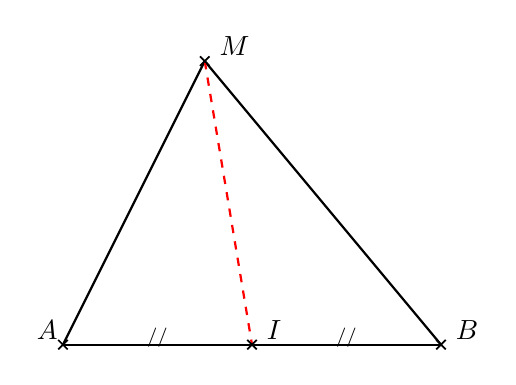
\begin{tikzpicture}[scale=1.2,>=stealth]

    % Définir les coordonnées des points A et B
    \coordinate (A) at (0,0);
    \coordinate (B) at (4,0);
    \coordinate (M) at (1.5,3);
    \coordinate (I) at (2,0);

    % Dessinez les vecteurs AB et AC
    \draw[thick,black] (A) -- (B) node[midway,anchor=south west] {};
    \draw[thick,black] (A) -- (M) node[midway,anchor=north west] {};
    \draw[thick,black] (M) -- (B) node[midway,anchor=north west] {};
    \draw[thick,red,dashed] (M) -- (I) node[midway,anchor=north west] {};

    % Ajouter des signes d'égalité pour les segments AI et IB
    \node at ($(0, 0.55)!0.5!(I)$)[anchor=north] {\scriptsize{//}};
    \node at ($(I)!0.5!(4, 0.55)$)[anchor=north] {\scriptsize{//}};

    % Marquer les points A, B et M avec des croix plus petites et plus épaisses
    \draw[line width=0.6pt] (A) ++(-0.05,-0.05) -- ++(0.1,0.1) (A) ++(-0.05,0.05) -- ++(0.1,-0.1) node[anchor=south east] {$A$};
    \draw[line width=0.6pt] (B) ++(-0.05,-0.05) -- ++(0.1,0.1) (B) ++(-0.05,0.05) -- ++(0.1,-0.1) node[anchor=south west] {$B$};
    \draw[line width=0.6pt] (M) ++(-0.05,-0.05) -- ++(0.1,0.1) (M) ++(-0.05,0.05) -- ++(0.1,-0.1) node[anchor=south west] {$M$};
    \draw[line width=0.6pt] (I) ++(-0.05,-0.05) -- ++(0.1,0.1) (I) ++(-0.05,0.05) -- ++(0.1,-0.1) node[anchor=south west] {$I$};
\end{tikzpicture}
\end{minipage}

\subsection*{2. Théorème d'Al Kashi}


\underline{Démonstration \emph{(théorème d'Al Kashi ou théorème de Pythagore généralisé ou loi des cosinus)} :}

\begin{minipage}{0.35\textwidth}
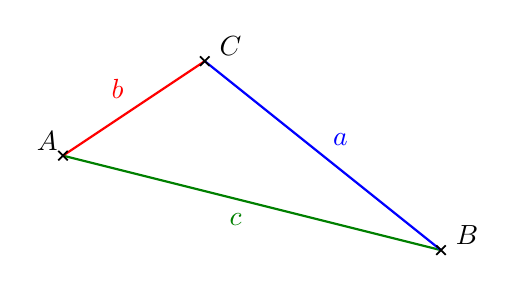
\begin{tikzpicture}[scale=1.2,>=stealth]

    % Définir les coordonnées des points A et B
    \coordinate (A) at (0,2);
    \coordinate (B) at (4,1);
    \coordinate (C) at (1.5,3);

    % Dessinez les vecteurs AB et AC
    \draw[dark_green, thick] (A) -- (B) node[midway,anchor=north east] {$c$};
    \draw[red, thick] (A) -- (C) node[midway,anchor=south east] {$b$};
    \draw[blue, thick] (C) -- (B) node[midway,anchor=south west] {$a$};

    % Marquer les points A, B et M avec des croix plus petites et plus épaisses
    \draw[line width=0.6pt] (A) ++(-0.05,-0.05) -- ++(0.1,0.1) (A) ++(-0.05,0.05) -- ++(0.1,-0.1) node[anchor=south east] {$A$};
    \draw[line width=0.6pt] (B) ++(-0.05,-0.05) -- ++(0.1,0.1) (B) ++(-0.05,0.05) -- ++(0.1,-0.1) node[anchor=south west] {$B$};
    \draw[line width=0.6pt] (C) ++(-0.05,-0.05) -- ++(0.1,0.1) (C) ++(-0.05,0.05) -- ++(0.1,-0.1) node[anchor=south west] {$C$};
\end{tikzpicture}
\end{minipage}
\hfill
\begin{minipage}{0.6\textwidth}
\begin{align*}
    \text{Calculons }a^2&=BC^2 \\
    &=\overrightarrow{BC}^2 \\
    &=(\overrightarrow{BA}+\overrightarrow{AC})^2 \\
    &=\|\overrightarrow{BA}\|^2+2\overrightarrow{BA}\pdt\overrightarrow{AC}+\|\overrightarrow{AC}\|^2 \\
    &=c^2+2(-\overrightarrow{AB})\pdt\overrightarrow{AC}+b^2 \\
    &=c^2-2\overrightarrow{AB}\pdt\overrightarrow{AC}+b^2 \\
    &=b^2+c^2-2bc\times\cos{(\widehat{A})}
\end{align*}
\end{minipage}

\subsection*{3. Caractérisation du cercle}

\underline{Démonstration :}
\begin{align*}
    \overrightarrow{MA}\pdt\overrightarrow{MB}=0&\Leftrightarrow MI^2-\frac{AB^2}{4}=0 \text{ avec $I$ milieu de $[AB]$} \\
    &\Leftrightarrow MI^2=\frac{AB^2}{4} \\
    &\Leftrightarrow MI = \sqrt{\frac{AB^2}{4}} \\
    &\Leftrightarrow MI = \frac{AB}{2} \\
    &\Leftrightarrow M \text{ appartient au cercle de centre $I$ et de rayon $\frac{AB}{2}$, c'est à dire au cercle de diamètre $[AB]$.} \\
\end{align*}

\end{document}
% ----- FIN DU DOCUMENT -----
